\section{Empirical Analysis}
%
We first discuss empirical results from the three-tanks running
example (see
figure~\ref{fig:three_tanks}). Figure~\ref{fig:fault_injection} shows
the results from one test case: a failure injection (valve $R_1$ stuck
at $50$\% at $t = 250$. For this simulation we use the highly accurate
non-linear model. The results from this simulation show that at the
time of the fault injection, the water level in tank $T_1$ starts
increasing while the water level at tanks $T_2$ and $T_3$ start
decreasing due to the smaller inflow.
%
\begin{figure}[htb]
  \centering
  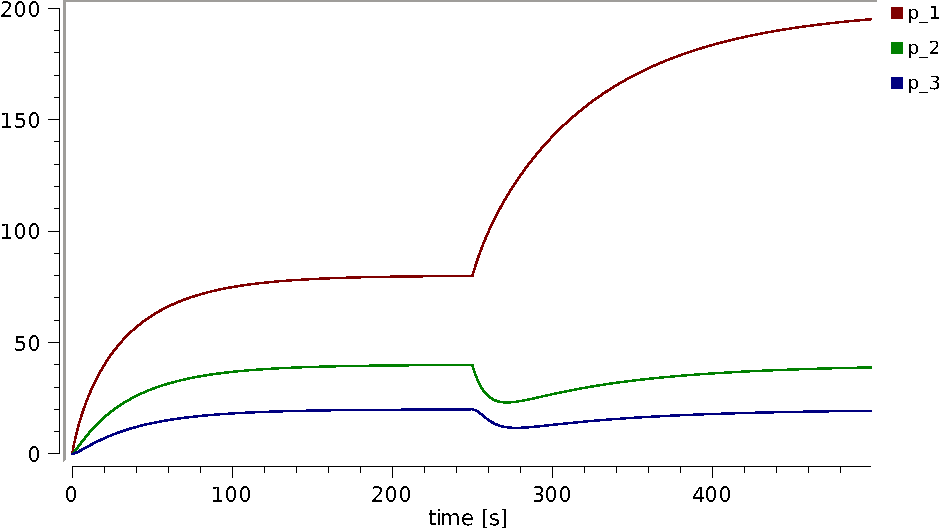
\includegraphics[scale=0.4]{fault_injection}
  \caption{Fault injection at $t = 250$~[s]}
  \label{fig:fault_injection}
\end{figure}
\par
%
We use the simulation output shown in figure~\ref{fig:three_tanks} to
create a test case for algorithm~\ref{alg:compose_model}. The result
of performing diagnosis with the same non-linear model (as used in
simulation) are shown in figure~\ref{fig:diagnosis}. We can see that
the diagnostic accuracy is high (the number of classification errors
at $t = 432$~[s] is only $M_{\mathrm{err}} = 0.034$). The isolation
accuracy is also very high ($M_{\mathrm{iso}} = 7$~[s]).
%
\begin{figure}[htb]
  \centering
  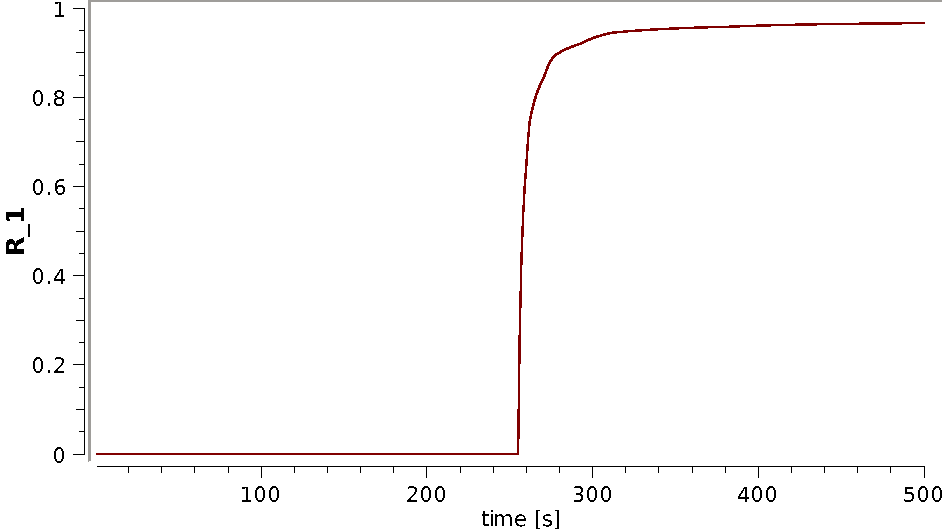
\includegraphics[scale=0.4]{diagnosis}
  \caption{Probability of $R_1$ being at fault with all components non-linear}
  \label{fig:diagnosis}
\end{figure}
\par
%
Figure~\ref{fig:diagnosis_linear_model} shows the diagnostic accuracy
and isolation time with an all-linear model. This all-linear model
delivers both bad diagnostic accuracy (classification errors) and bad
isolation time. After the fault injection at $t = 250$~[s] the
probability estimation is better and the fault valve, at-least appears
at the top of the list of faulty components. The benefit of the
all-linear model is that it is much faster to simulate.
%
\begin{figure}[htb]
  \centering
  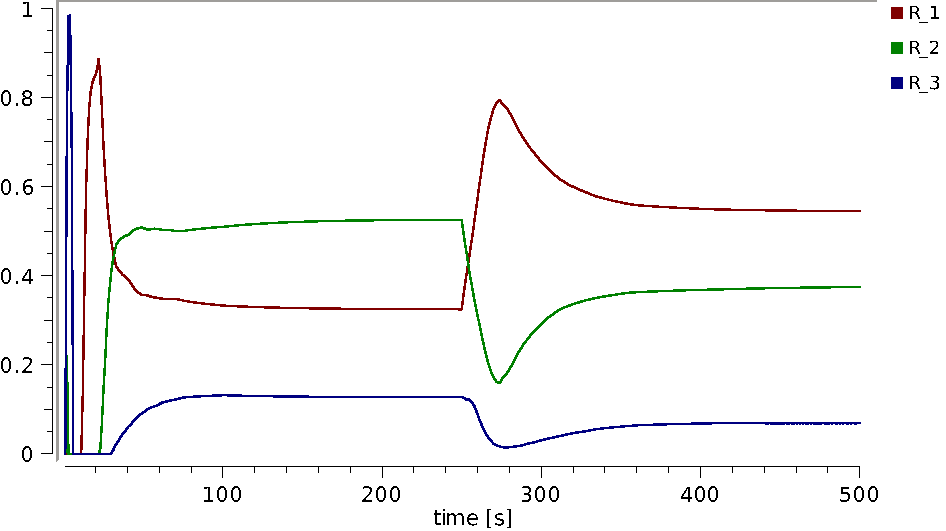
\includegraphics[scale=0.4]{diagnosis_linear_model}
  \caption{Probability of $R_1, R_2$, and $R_3$ being at fault with all components linear}
  \label{fig:diagnosis_linear_model}
\end{figure}
\par
%
The plot in figure~\ref{fig:diagnosis_t2_t3_linear} shows the
diagnostic performance with partly linear, partly non-linear model
($T_1$ is non-linear, while $T_2$ and $T_3$ are linear). The
diagnostic accuracy is almost the same, except a false-positive
detection in the beginning of the scenario which we are ignoring. Of
course, the number of computations for simulating the partly linear
model is significantly smaller (recall that we need multiple
simulations for diagnosis). As a result this model is a preferred
compromise for diagnostic accuracy and computational complexity.
%
\begin{figure}[htb]
  \centering
  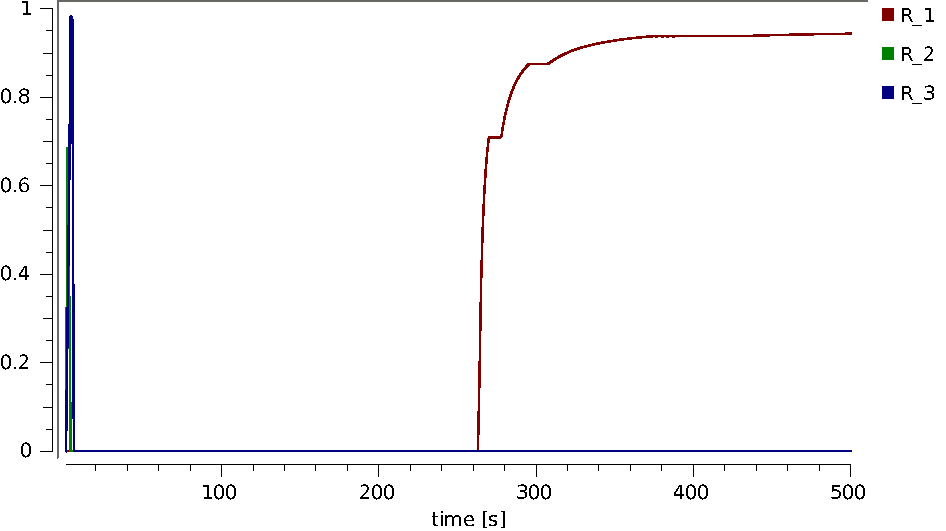
\includegraphics[scale=0.4]{diagnosis_t2_t3_linear}
  \caption{Probability of $R_1, R_2$, and $R_3$ being at fault with $T_1$ non-linear and both $T_2$ and $T_3$ linear}
  \label{fig:diagnosis_t2_t3_linear}
\end{figure}
\par
%
Algorithm~\ref{alg:compose_model} is insensitive to the cardinality of
the fault injection. Figure~\ref{fig:double_fault_injection}, for
example, shows the result of a double-fault injection. The first fault
is a $50$~\%-stuck valve $R_1$ at $t = 250$ and the second fault is a
stuck-valve $R_2$ at $75$~\% at $t = 250$. Clearly, the effect of the
second fault is less pronounced due to its magnitude.
%
\begin{figure}[htb]
  \centering
  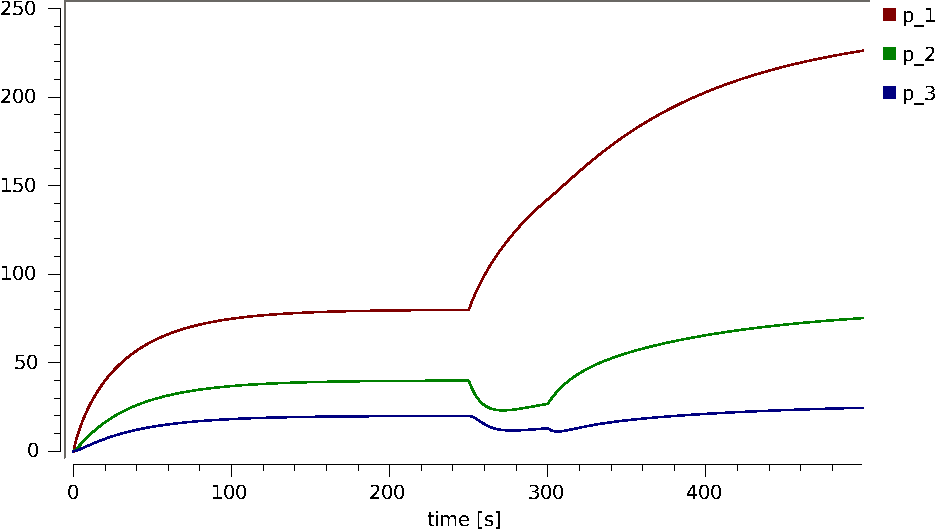
\includegraphics[scale=0.4]{double_fault_injection}
  \caption{Fault injection of a double fault at $t = 250$~[s] and $t = 300$~[s]}
  \label{fig:double_fault_injection}
\end{figure}
\par
Figure~\ref{fig:diagnosis_double} shows the fault-probability for the
double-fault injection shown in
figure~\ref{fig:double_fault_injection} with a fully non-linear
model. For this, we have configured the diagnostic reasoner to
consider double-fault hypotheses (see \cite{feldman13genius}). Both
faults are captured with short isolation time. The first
classification errors metrics is $M_{\mathrm{err}} = 0$ and
$M_{\mathrm{iso}} = 9$ while for the second (cumulative) fault we have
$M_{\mathrm{err}} = 0.445$ and $M_{\mathrm{iso}} = 31$.
%
\begin{figure}[htb]
  \centering
  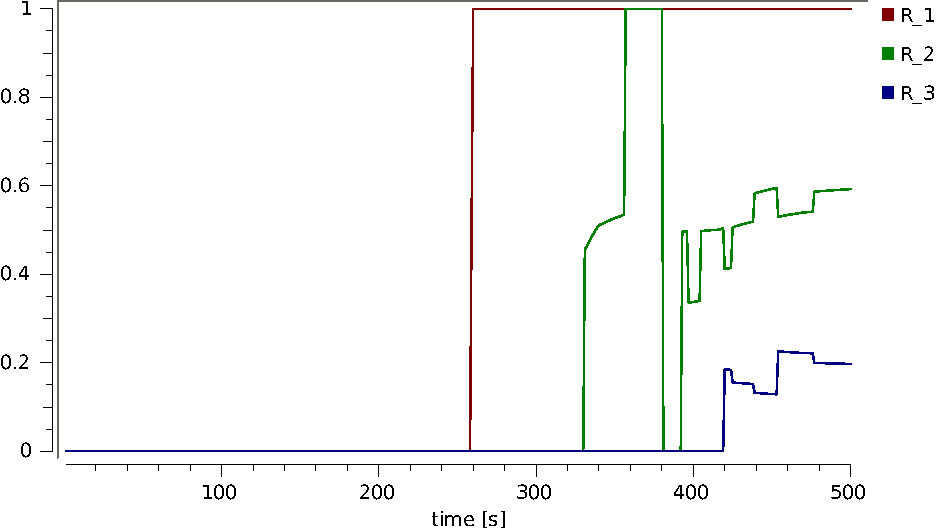
\includegraphics[scale=0.4]{diagnosis_double}
  \caption{Probability of finding the double-fault with all components non-linear}
  \label{fig:diagnosis_double}
\end{figure}
\par
Figure~\ref{fig:diagnosis_double_t2_t3_linear} shows the diagnostic
performance of the model computed by
algorithm~\ref{alg:compose_model}. In this model tank equations for
$T_1$ are non-linear while tank equations for $T_2$ and $T_3$ are
linear. The diagnostic performance 
%
\begin{figure}[htb]
  \centering
  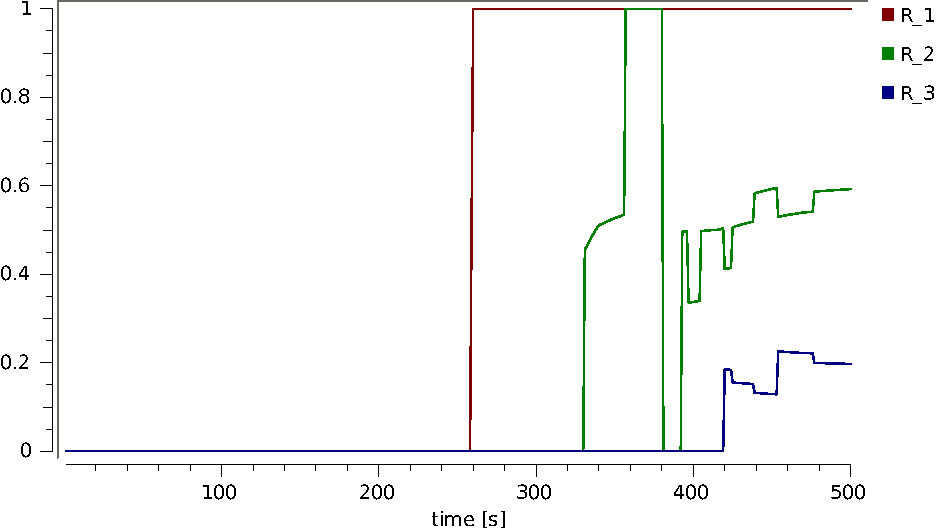
\includegraphics[scale=0.4]{diagnosis_double_t2_t3_linear}
  \caption{Probability of discovering an $R_1$ and $R_2$ double-fault with $T_1$ non-linear and both $T_2$ and $T_3$ linear}
  \label{fig:diagnosis_double_t2_t3_linear}
\end{figure}
\par
%
Again, the partly-linear model whose performance is shown in
figure~\ref{fig:diagnosis_double_t2_t3_linear} is the best
compromise in terms of diagnostic accuracy and computational
efficiency.
\par
The results from all our experiments are non-intuitive in a sense that
if we replace a non-linear component model with a linear one it does
not affect the diagnostic accuracy while it improves other
metrics. This cannot be done mechanically for all components as the
diagnostic accuracy may deteriorate suddenly. This all makes us believe
that the role of the topology for diagnostic reasoning is important.
